\subsection{Graphing Lines from Points}\pp

 {\tmstrong{Objective: Graph lines using $xy$-coordinates.}}\pp

 The main purpose of graphs is not to plot random points, but rather to give a
picture of the solutions to an equation. We may have an equation such as $y =
2 x - 3$. We may be interested in what type of solution are possible in this
equation. We can visualize the solution by making a graph of possible $x
\tmop{and} y$ combinations that make this equation a true statement. We will
have to start by finding possible $x \tmop{and} y$ combinations. We will do
this using a table of values.

\begin{example}\label{Lin44}
  \begin{eqnarray*}
    \tmop{Graph} y = 2 x - 3 &  & \tmop{We} \tmop{make~a} \tmop{table}
    \tmop{of} \tmop{values}\\
    &  & \\
    \begin{array}{|c|c|}
      \hline
      x & ~~y~~\\
      \hline
      - 1 & \\
      \hline
      0 & \\
      \hline
      1 & \\
      \hline
    \end{array} &  & \tmop{We} \tmop{will} \tmop{test} \tmop{three}
    \tmop{values} \tmop{for} x. \tmop{Any} \tmop{three} \tmop{can} \tmop{be}
    \tmop{used}\\
    &  & \\
    \begin{array}{|c|c|}
      \hline
      x & y\\
      \hline
      - 1 & - 5\\
      \hline
      0 & - 3\\
      \hline
      1 & - 1\\
      \hline
    \end{array} &  & \begin{array}{l}
      \tmop{Evaluate} \tmop{each} \tmop{by} \tmop{replacing} x \tmop{with}
      \tmop{the} \tmop{given} \tmop{value}\\
      x = - 1 ~~~~~~~ y = 2 (- 1) - 3 = - 2 - 3 = - 5\\
      x = 0  ~~~~~~~~~y = 2 (0) - 3 = 0 - 3 = - 3\\
      x = 1  ~~~~~~~~~y = 2 (1) - 3 = 2 - 3 = - 1
    \end{array}\\
    &  & \\
    (- 1, - 5), (0, - 3), (1, - 1) &  & \tmop{These} \tmop{then} \tmop{become}
    \tmop{the} \tmop{points} \tmop{to} \tmop{graph} \tmop{on} \tmop{our}
    \tmop{equation}
  \end{eqnarray*}
  \begin{multicols}{2}
    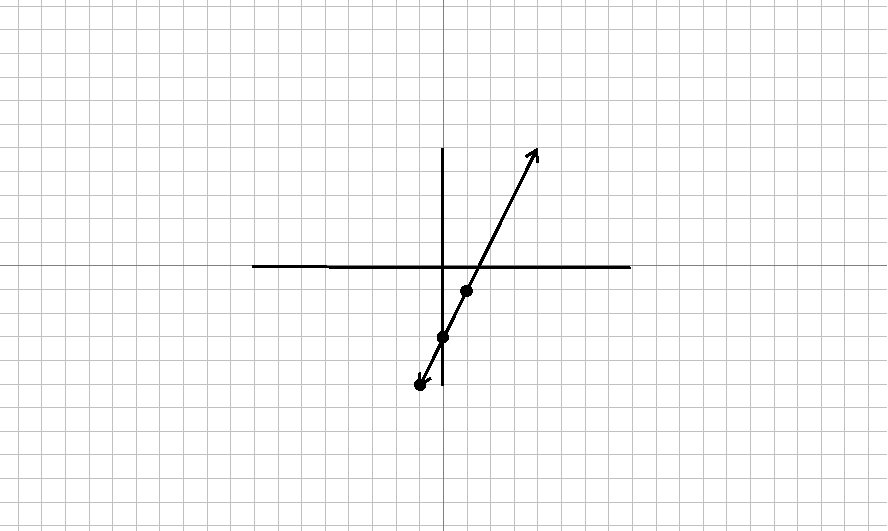
\includegraphics[scale=.9,bb = 115 65 310 190, clip=true]{II_1_3b-7.eps}
    
    \
    
     Plot each point.\\
    
     Once the point are on the graph, connect the dots to make a line.\\
    
     The graph is our solution.
  \end{multicols}
\end{example}

 What this line tells us is that any point on the line will work in the
equation $y = 2 x - 3$. For example, notice the graph also goes through the
point $(2, 1)$. If we use $x = 2$, we should get $y = 1$. Sure enough, $y = 2
(2) - 3 = 4 - 3 = 1$, just as the graph suggests. Thus we have the line is a
picture of all the solutions for $y = 2 x - 3$. We can use this table of
values method to draw a graph of any linear equation.

\begin{example}\label{Lin45}
  
  \begin{eqnarray*}
    \tmop{Graph} 2 x - 3 y = 6 &  & \tmop{We} \tmop{will} \tmop{use} \tmop{a}
    \tmop{table} \tmop{of} \tmop{values}\\
    &  & \\
    \begin{array}{|c|c|}
      \hline
      x & ~y~~\\
      \hline
      - 3 & \\
      \hline
      0 & \\
      \hline
      3 & \\
      \hline
    \end{array} &  & \tmop{We} \tmop{will} \tmop{test} \tmop{three}
    \tmop{values} \tmop{for} x. \tmop{~Any} \tmop{three} \tmop{can} \tmop{be}
    \tmop{used}.\\
    %&  & \\
      \end{eqnarray*}
      \begin{eqnarray*}
		2 (- 3) - 3 y = 6~ &  & \tmop{Substitute} \tmop{each} \tmop{value}
    \tmop{in} \tmop{for} x \tmop{and} \tmop{solve} \tmop{for} y\\
    - 6 - 3 y = 6~ &  & \tmop{Start} \tmop{with} x = - 3, \tmop{multiply}
    \tmop{first}\\
    \bf{\underline{+ 6 ~~~~~~~+ 6}} &  & \tmop{Add} 6 \tmop{to} \tmop{both} \tmop{sides}\\
    - 3 y = 12~ &  & \tmop{Divide} \tmop{both} \tmop{sides} \tmop{by} - 3\\
    \bf{\overline{- 3} ~~~ \overline{- 3}}~ &  & \\
    y = - 4~ &  & \tmop{solution} \tmop{for} y \tmop{when} x = - 3, \tmop{add}
    \tmop{this} \tmop{to} \tmop{table}\\
    &  & \\
    2 (0) - 3 y = 6~ &  & \tmop{Next} x = 0\\
    - 3 y = 6~ &  & \tmop{Multiplying} \tmop{clears} \tmop{the} \tmop{constant}
    \tmop{term}\\
    \bf{\overline{- 3} ~~~~ \overline{- 3}} &  & \tmop{Divide} \tmop{each} \tmop{side}
    \tmop{by} - 3\\
    y = - 2~ &  & \tmop{solution} \tmop{for} y \tmop{when} x = 0, \tmop{add}
    \tmop{this} \tmop{to} \tmop{table}\\
    &  & \\
    2 (3) - 3 y = 6~ &  & \tmop{Next} x = 3\\
    6 - 3 y = 6~ &  & \tmop{Multiply}\\
    \bf{\underline{- 6 ~~~~~~~~- 6}} &  & \tmop{Subtract} 9 \tmop{from} \tmop{both}
    \tmop{sides}\\
    - 3 y = 0~ &  & \tmop{Divide} \tmop{each} \tmop{side} \tmop{by} - 3\\
    \bf{\overline{- 3} ~~~ \overline{- 3}} &  & \\
    y = 0~ &  & \tmop{solution} \tmop{for} y \tmop{when} x = - 3, \tmop{add}
    \tmop{this} \tmop{to} \tmop{table}\\
    &  & \\
      \end{eqnarray*}
      \begin{eqnarray*}
		\begin{array}{|c|c|}
      \hline
      x & y\\
      \hline
      - 3 & - 4\\
      \hline
      0 & - 2\\
      \hline
      3 & 0\\
      \hline
    \end{array} &  & \tmop{Our} \tmop{completed} \tmop{table}\\
    &  & \\
    (- 3, - 4), (0, 2), (3, 0) &  & \tmop{Coordinate} \tmop{points} \tmop{from}
    \tmop{table}
  \end{eqnarray*}
  \begin{multicols}{2}
    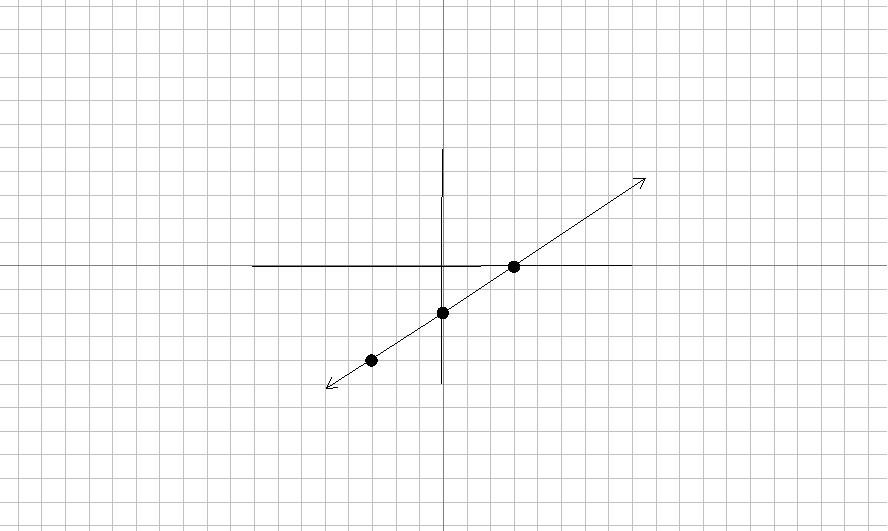
\includegraphics[scale=.9,bb = 115 65 310 190, clip=true]{II_1_3b-8.eps}
    
    \
    
     Graph points and connect dots
    
    \
    
     Our solution
  \end{multicols}
\end{example}